\documentclass[11pt,a4paper]{scrartcl}
\usepackage[utf8]{inputenc}
\usepackage[italian]{babel}

\usepackage{amsmath, amsfonts, amssymb}
\usepackage{graphicx, booktabs}
\usepackage{minted}

\usepackage{multirow}
\usepackage{parskip}

\author{L. De Sano, A. Donizetti, M. Scotti}
\title{La trasformata DCT applicata alle immagini}
\date{Giugno 2014}

\begin{document}
\maketitle
\begin{abstract}
Descriviamo l'implementazione di una serie di test riguardanti l'applicazione della trasformata DCT2 ad immagini bitmap \textit{grayscale}, il taglio di alcune delle frequenze della trasformata, l'applicazione della IDCT2 alla matrice risultante, e il confronto con l'originale dell'immagine bitmap ottenuta dopo il taglio.
\end{abstract}

\section*{Implementazione}

In questa sezione diamo una descrizione dell'implementazione dei test richiesti dalla consegna. Le parti di lettura file BMP, calcolo DCT2 e IDCT2, taglio delle frequenze, e ri-esportazione dell'immagine sono scritte in C99 (compilato come C++ per via della dipendenza da una libreria per la manipolazione di immagini da noi utilizzata, scritta in C++). Il codice che disegna e stampa a schermo l'istogramma delle frequenze è scritto in Python.

\subsection*{Lettura delle immagini}

Le immagini campione fornite su \texttt{k.matapp.unimib.it} non sono memorizzate come BMP pure e senza compressione (ovvero: il file non contiene semplicemente una matrice con i valori in \emph{greyscale} dei pixel), ma sono compresse usando una \emph{run-length encoding} a 8 bits. Per questo motivo abbiamo scartato l'idea di scrivere a mano un lettore di files BMP, e deciso di utilizzare una libreria esterna (possibilmente il più leggera possibile) per l'importazione delle immagini.

Una libreria di semplice utilizzo che abbiamo trovato è CImg\footnote{cimg.sourceforge.net}, scritta in C++. Non richiede installazione, e consiste in un unico \emph{header file} \texttt{CImg.h} che va semplicemente incluso nella \emph{directory} del progetto. L'utilizzo di una libreria C++ ci ha costretti a compilare il resto del nostro codice (C99 puro) come C++, ma le differenze tra i due linguaggi sono minimali e gli adattamenti che abbiamo dovuto fare sul codice già scritto sono stati di poco conto.

Il codice (C++) utilizzato per la lettura dell'immagine è il seguente:

\begin{minted}[frame=single]{c++}
CImg<uint8_t> image(argv[1]);   // argv[1] contiene il nome del file
uint8_t * img = image.data();   // i dati rilevanti salvati in un array
int m = image.height();         // estraendo poi dall'header altezza
int n = image.width();          //         e larghezza dell'immagine
\end{minted}

Da notare che la matrice che contiene i pixel è di tipo \texttt{uint8\_t}, dato che la consegna del progetto richiedeva di operare esclusivamente su immagini \emph{greyscale}. CImg è in grado di leggere senza problemi immagini BMP compresse con RLE, e i dati ritornati dal metodo \texttt{data( )} rappresentano i pixel già scompattati.

\subsection*{DCT2}

Scrivendo in C99, è banale chiamare direttamente FFTW3. La libreria è facile da installare e ben documentata. La chiamata avviene in due passaggi: prima di tutto si crea un piano (\emph{plan}) con le caratteristiche della FT che si vuole operare sui dati, successivamente lo si esegue.

Le funzione FFTW3 da utilizzare per la creazione di un \emph{plan} DCT2 da $\mathbb{R}^2$ ad $\mathbb{R}^2$ è \texttt{fftw\_plan\_r2r\_2d( )}. Alla funzione, oltre che i parametri con i dati da trasformare, vanno passate due flag (una per ognuna delle due dimensioni) che specificano quale tipo di trasformata applicare. Nel nostro caso, per entrambe, si tratta di \texttt{FFTW\_REDFT10}:

FFTW\_REDFT10 (DCT-II, 'the' DCT):
\begin{quotation}
even around $j=-0.5$ and even around $j=n-0.5$
\end{quotation}

\begin{minted}[frame=single]{c}
double * dct2(int m, int n, uint8_t * array)
{
    // setup input e output
    double * out = (double *) malloc(sizeof(double) * m * n);
    double * in  = to_double(m, n, array);

    // do the fftw3 magic
    fftw_plan plan = fftw_plan_r2r_2d(m, n, in, out, FFTW_REDFT10,
				      FFTW_REDFT10, FFTW_ESTIMATE);
    fftw_execute(plan);

    // normalizzazione
    normalizza(m, n, out);
    return out;
}
\end{minted}

La funzione \texttt{dct2} prende un array di \texttt{uint8\_t} e restituisce un array di \texttt{double} contenente la DCT2 dell'input normalizzata, come richiesto, per replicare i risultati della funzione \texttt{dct2} di Matlab.

La funzione di normalizzazione è implementata come indicato nella consegna:

\begin{minted}[frame=single]{c}
void normalizza(int m, int n, double * array)
{
    double norm1 = 4 * sqrt(m/2.0) * sqrt(n/2.0);
    double norm2 = sqrt(2);
    
    for(int i = 0; i < m; i++){            // globale
        for(int j = 0; j < n; j++)
            array[i*n + j] /= norm1;     
    }

    for(int i = 0; i < n; i++)            // prima riga
        array[i] /= norm2;

    for(int j = 0; j < (m*n); j+=n)       // prima colonna
        array[j] /= norm2;
}
\end{minted}

\subsection*{Calcolo Istogrammi}
Per il calcolo degli istogrammi, una funzione \texttt{hist( )} accetta come parametro il numero di \emph{bins} e dopo averne calcolato la larghezza (basandosi sul valore massimo contenuto nella DCT), conteggia, per ognuno dei \emph{bins}, il numero di coefficienti presenti all'interno del \emph{bin}.

\begin{minted}[frame=single]{c}
void hist(int m, int n, int bins, double * array, const char * name)
{
    double max; // il valore massimo in array
    /* calcola max */
   
    double bins_width = (max + 100.0) / bins;
    int * hist = calloc(bins, sizeof(int));
    for(int i = 0; i < m; i++){
        for(int j = 0; j < n; j++)
	        hist[ (int)abs(array[i*n + j] / bins_width) ]++;
    }

    // continua ...
\end{minted}

\texttt{hist( )} salva su poi su file il risultato della computazione:
\begin{minted}[frame=single]{c}
    // ... continua
   
    FILE * fileptr = fopen(name, "w");
    fprintf(fileptr, "bins\t%d \n", bins);
    fprintf(fileptr, "width\t%.3f \n", bins_width);
    fprintf(fileptr, "max\t%.3f \n", max);
    for(int i = 0; i < bins; i++)
	fprintf(fileptr, "%d\n", hist[i]);

    fclose(fileptr);
}
\end{minted}


\subsection*{Taglio delle frequenze}

Dopo la visualizzazione dell'istogramma delle frequenze, l'utente può specificare un valore di soglia per il taglio della DCT2: ogni componente che sia in valore assoluto minore del valore di soglia è portata a zero.


\begin{minted}[frame=single]{c}
void cut_dct(int m, int n, double val, double * array)
{
    for(int i = 0; i < m; i++){
        for(int j = 0; j < n; j++){
            if(abs(array[i*n + j]) < val)
                array[i*n + j] = 0.0;
        }
    }
}
\end{minted}

La modifica è fatta, per ragioni di efficienza, \emph{in-place}: l'array originale viene perso e i valori originali sovrascritti in memoria.

\subsection*{IDCT2}

La funzione che opera il calcolo della IDCT2 è simile alla \texttt{dct2( )}. Per la creazione del piano è necessario passare come flag DCT \texttt{FFTW\_REDFT01} (che è l'inversa della \texttt{FFTW\_REDFT10} usata in precedenza per la DCT2), mentre la denormalizzazione divide per quello che la normalizzazione ha moltiplicato.

Dopo la denormalizzazione e il calcolo della IDCT2 (di cui non riportiamo il codice, essendo questo del tutto analogo a quello della \texttt{dct2( )} precedentemente descritta), è necessario applicare una trasformazione ulteriore. Infatti (citando dalla documentazione della FFTW3):
\begin{quotation}
the transforms computed by FFTW are unnormalized, exactly like the corresponding real and complex DFTs, so computing a transform followed by its inverse yields the original array scaled by $N$, where $N$ is the logical DFT size. For REDFT01, $N=2n$. 
\end{quotation}

Nel caso bidimensionale, il fattore di scala è $2n \cdot 2m = 4nm$, e va applicato dopo la denormalizzazione e  il calcolo della IDCT2.

\begin{minted}[frame=single]{c}
void scala(int m, int n, double * array)
{
    double scale = 4.0 * m * n;

    for(int i = 0; i < m; i++){
        for(int j = 0; j < n; j++)
            array[i*n + j] = array[i*n + j] / scale;
    }
}
\end{minted}

Senza questo passaggio, non è possibile confrontare direttamente la matrice \texttt{uint8\_t} di partenza e il risultato della IDCT2 (tralasciando in questo momento la questione taglio frequenze, che ovviamente va a modificare la matrice di partenza).

\subsection*{Esportazione delle immagini}
Per l'esportazione delle immagini tagliate utilizziamo ancora la CImg citata in precedenza. Il codice (C++):
\begin{minted}[frame=single]{c++}
CImg<uint8_t> image2(img2, n, m, 1, 1);
image2.save(strcat(argv[1], "cut.bmp"), -1, 3);;
\end{minted}

Nella prima riga viene costruito un oggetto CImg (\texttt{image2}) a partire dalla matrice dei pixel risultato della IDCT2 (\texttt{img2}). Nella seconda riga l'oggetto viene salvato su file con suffisso ``cut'' nel nome.

\section*{Risultati dei test}

Diamo un esempio di esecuzione del codice, usando l'immagine \texttt{flower\_foveon}, presa dall'insieme di test. Si tratta di un file BMP $2268 \times 1512$, codificato usando il livello di compressione 1 (RLE a 8 bit). La frequenza di taglio è 30 per la prima immagine (con il paragone di un dettaglio del fiore) e di 100 per il confronto sull'immagine completa.

\begin{figure}[!ht]
\centering
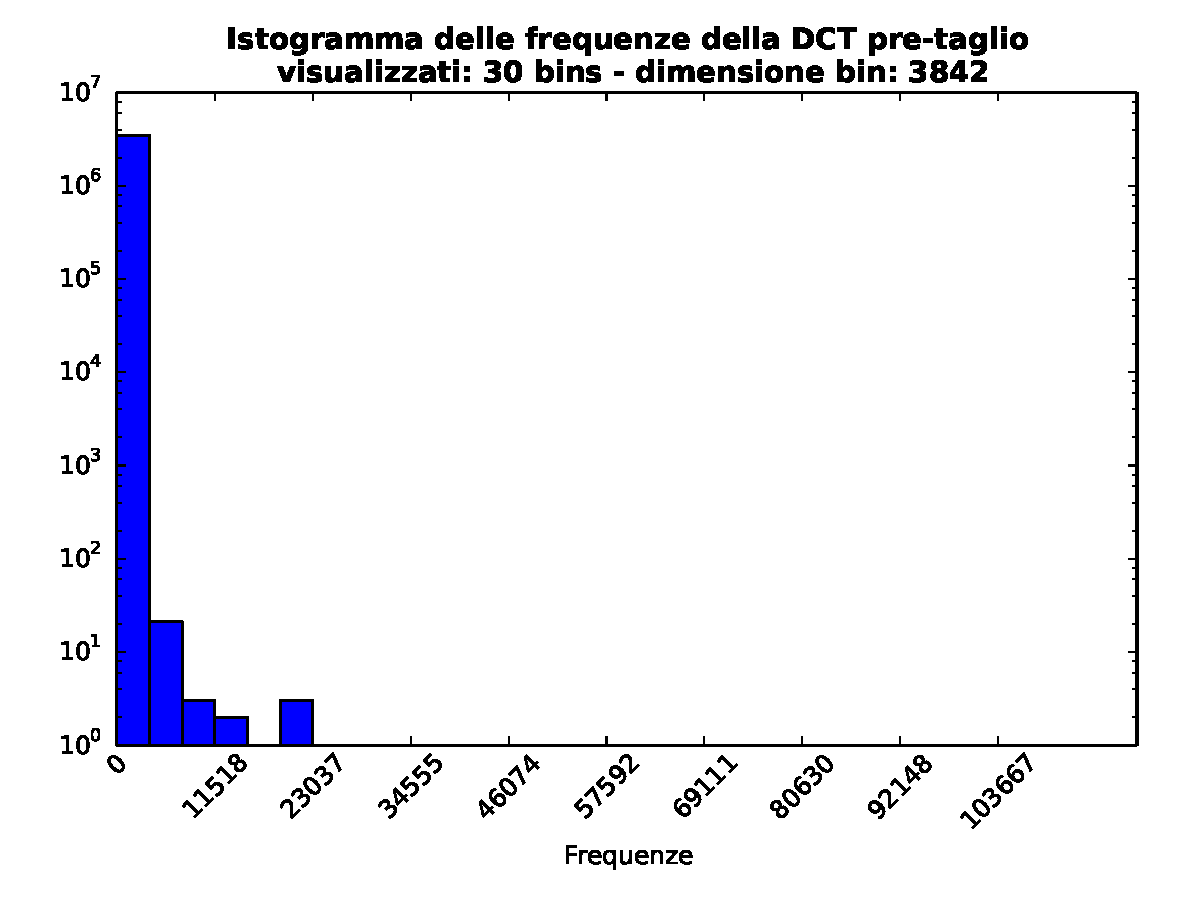
\includegraphics[scale=0.6]{images/hist_fiore_30_pre} 
\caption{\texttt{flower\_feveon.bmp}, istogramma frequenze della trasformata}
\end{figure}

\begin{figure}[!ht]
\centering
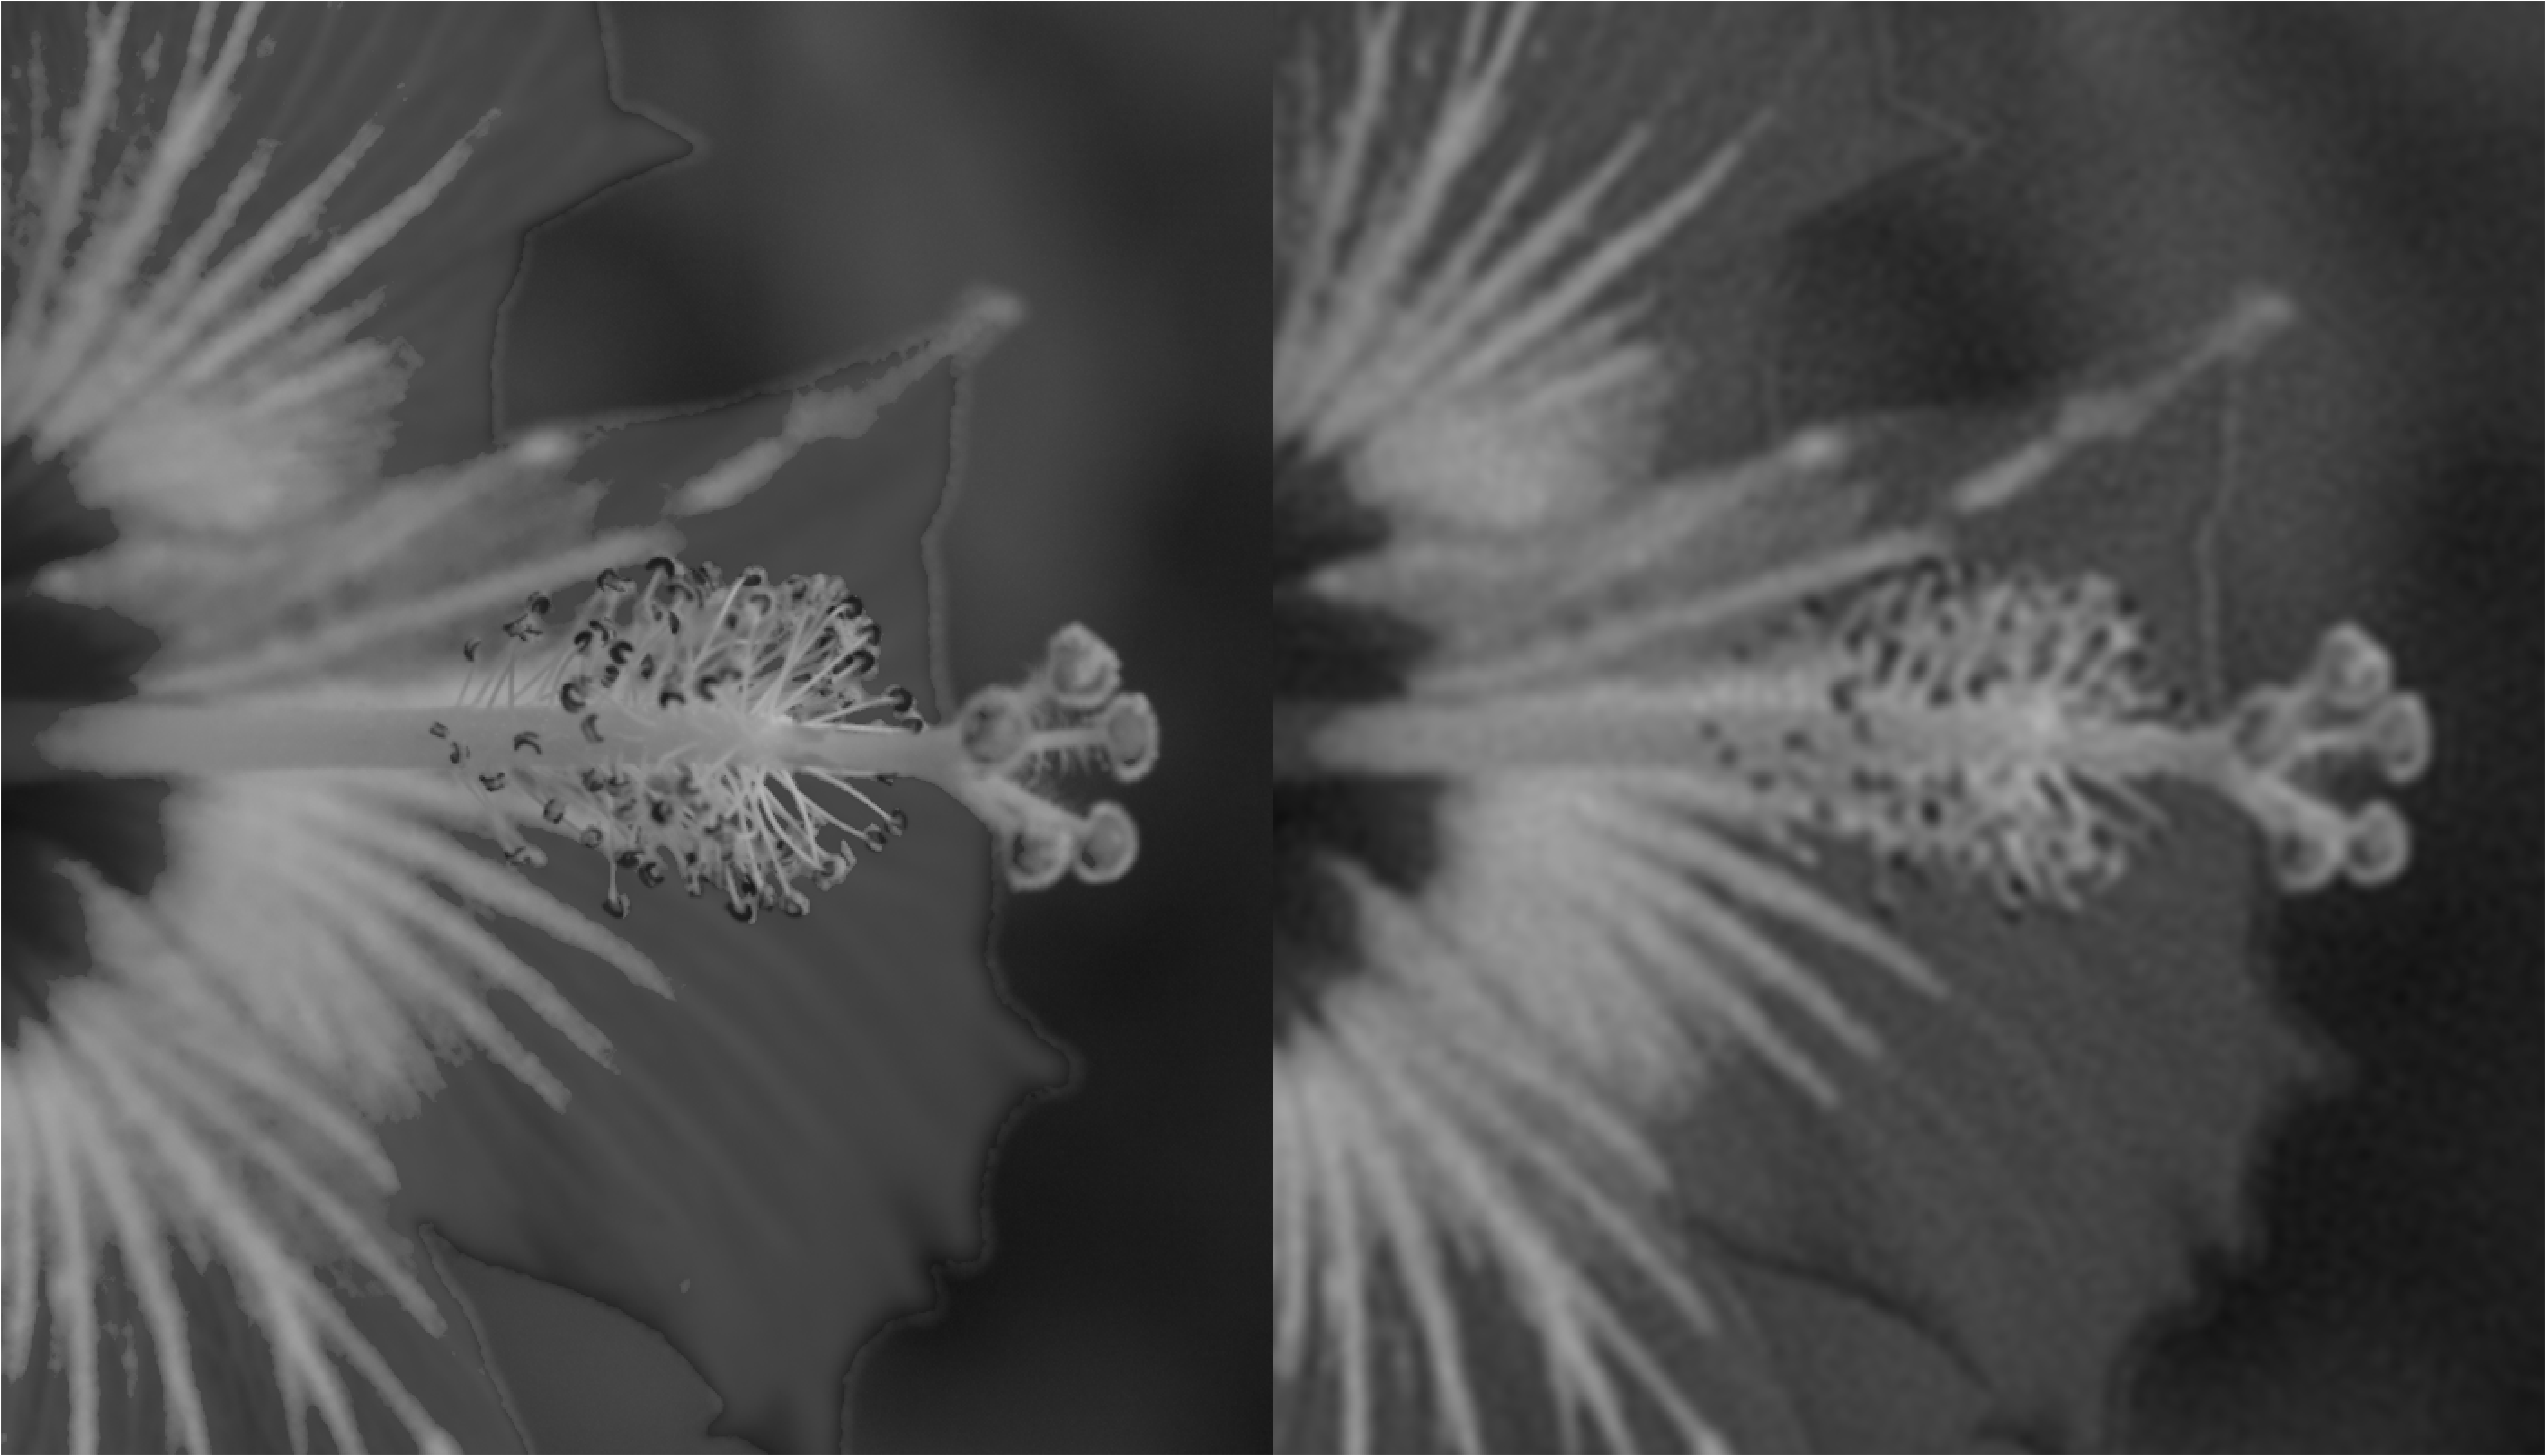
\includegraphics[scale=0.026]{images/cfr} 
\caption{\texttt{flower\_feveon.bmp}, particolare. Originale vs taglio frequenze $< 30$}
\end{figure}

\begin{figure}[!ht]
\centering
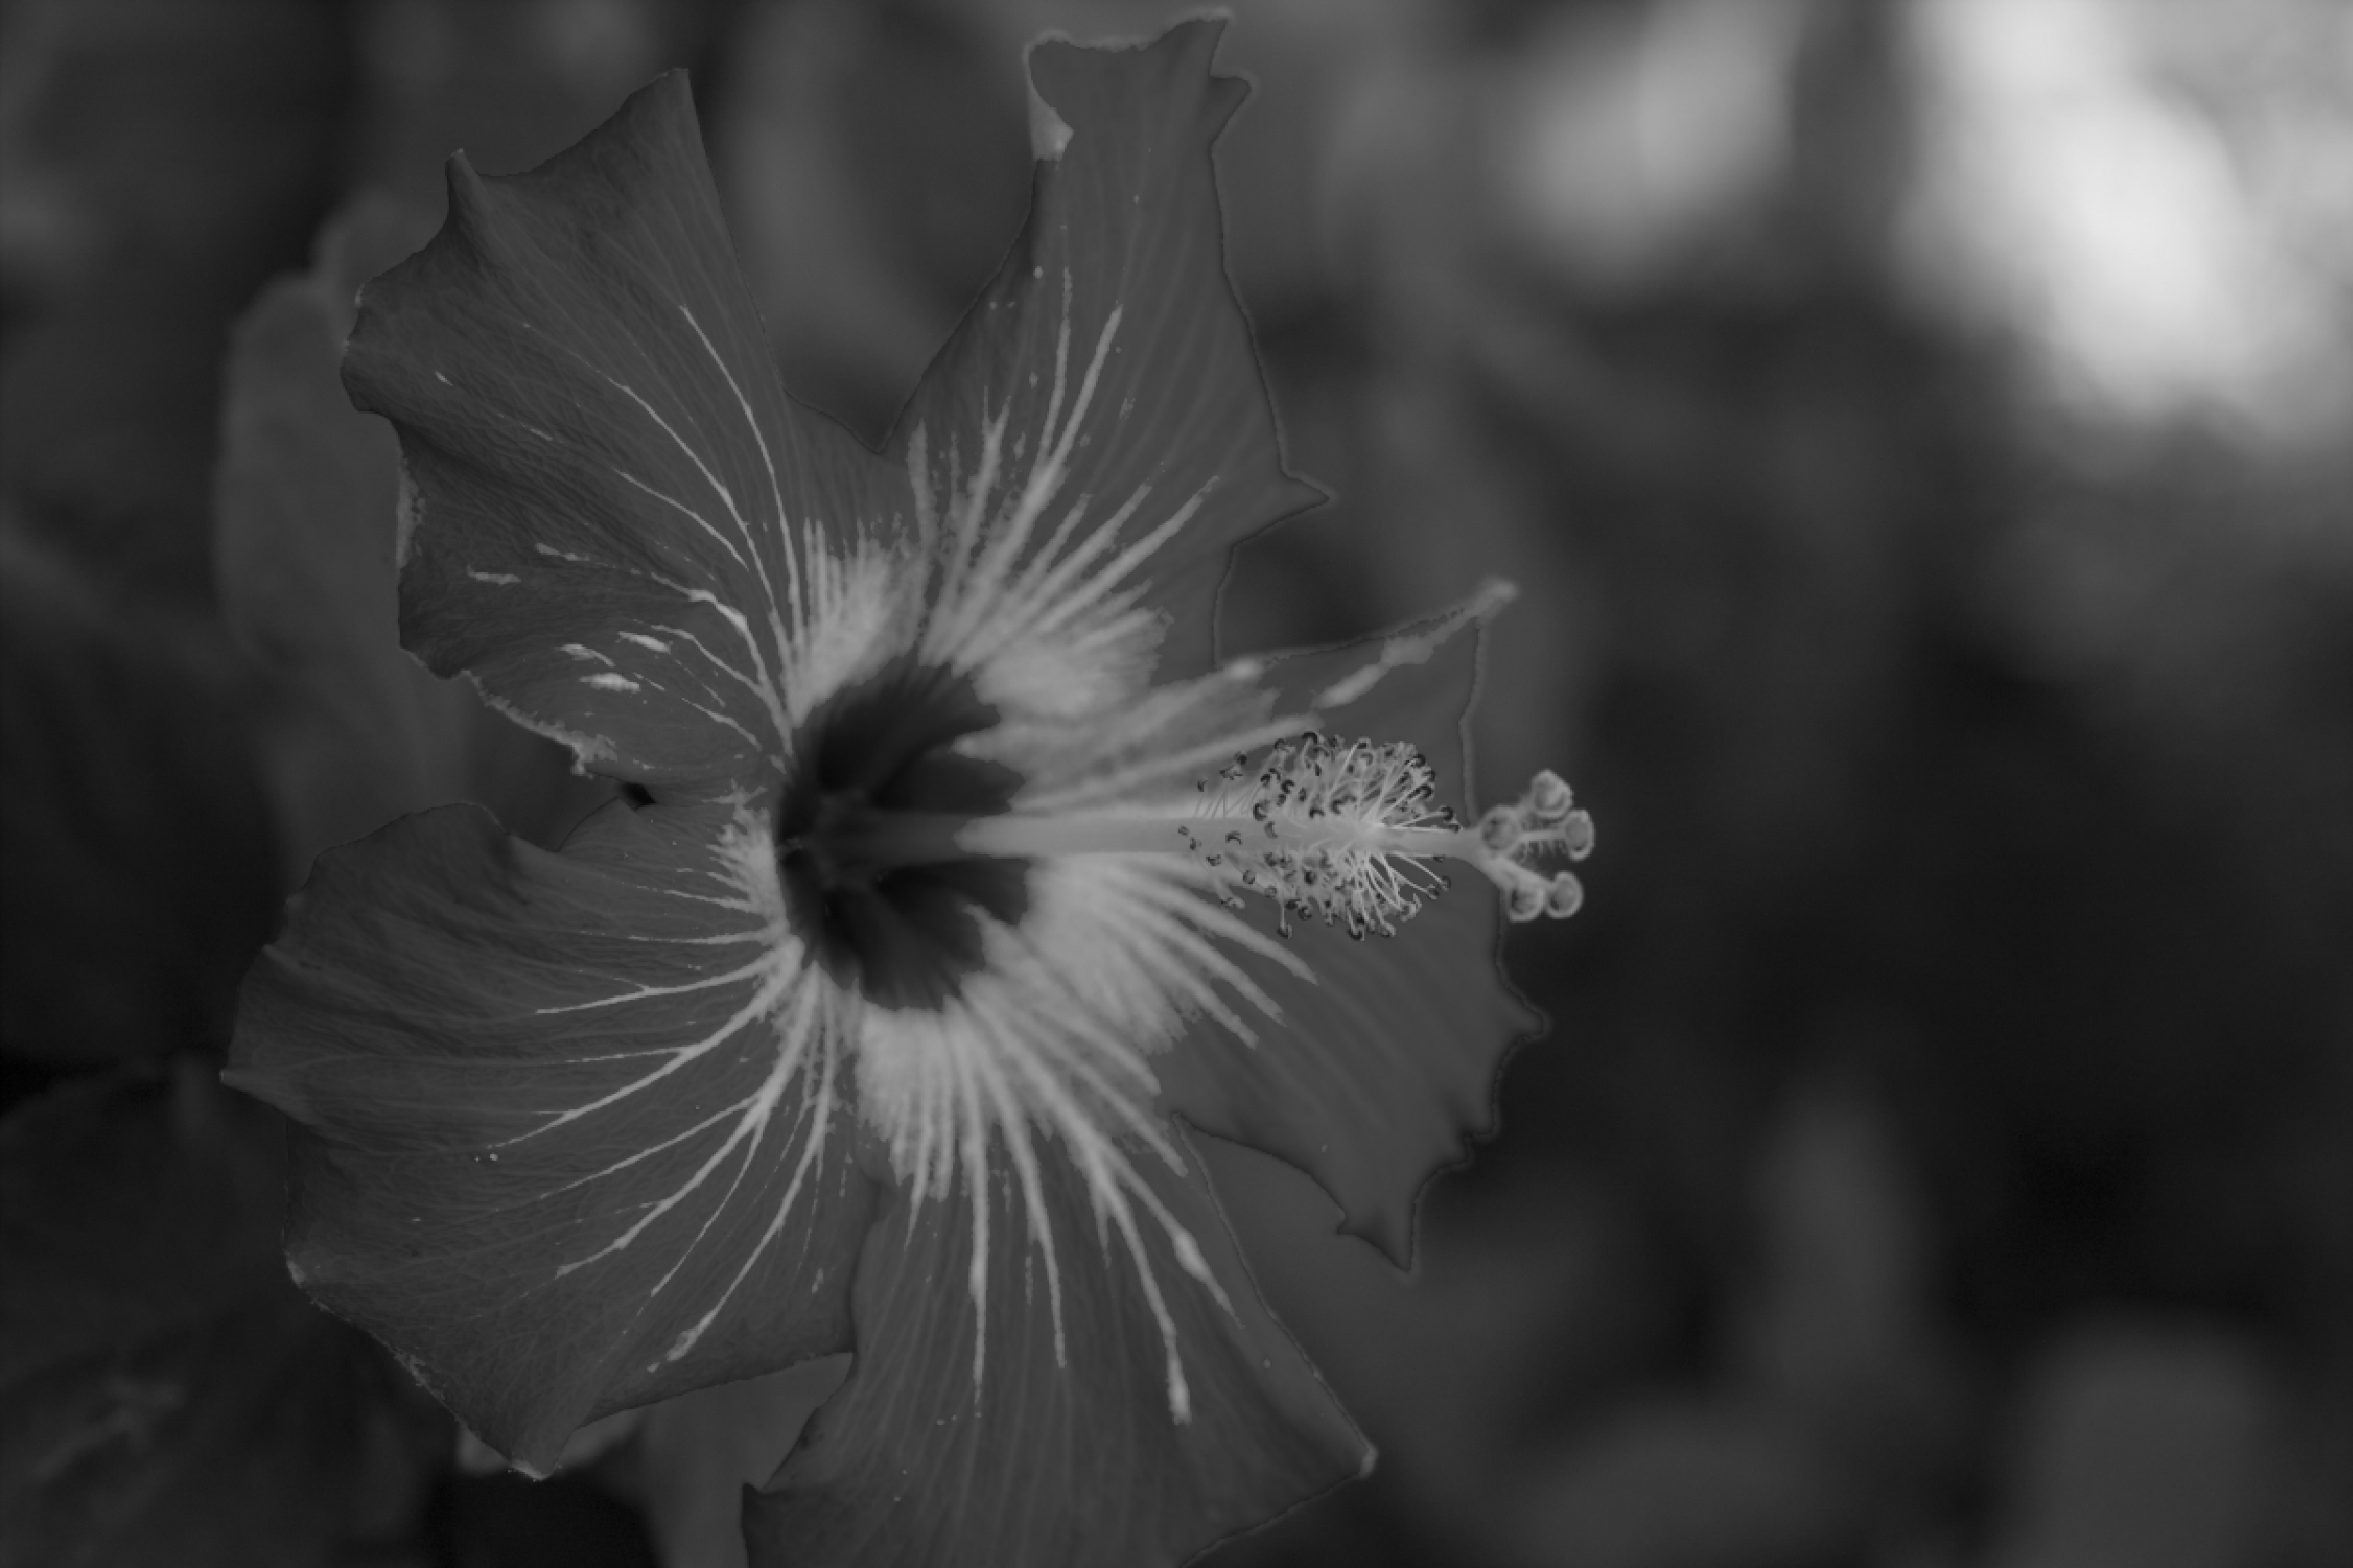
\includegraphics[scale=0.29]{images/flower_foveon} 
\caption{\texttt{flower\_feveon.bmp}, originale}
\end{figure}

\begin{figure}[!ht]
\centering
\includegraphics[scale=0.026]{images/flower_foveon_cut} 
\caption{\texttt{flower\_feveon.bmp}, taglio frequenze $< 100$}
\end{figure}

Un altro esempio, tagliando stavolta tutte le frequenze in valore assoluto minori di 5000 sull'immagine \texttt{big\_building}:

\begin{figure}[!ht]
\centering
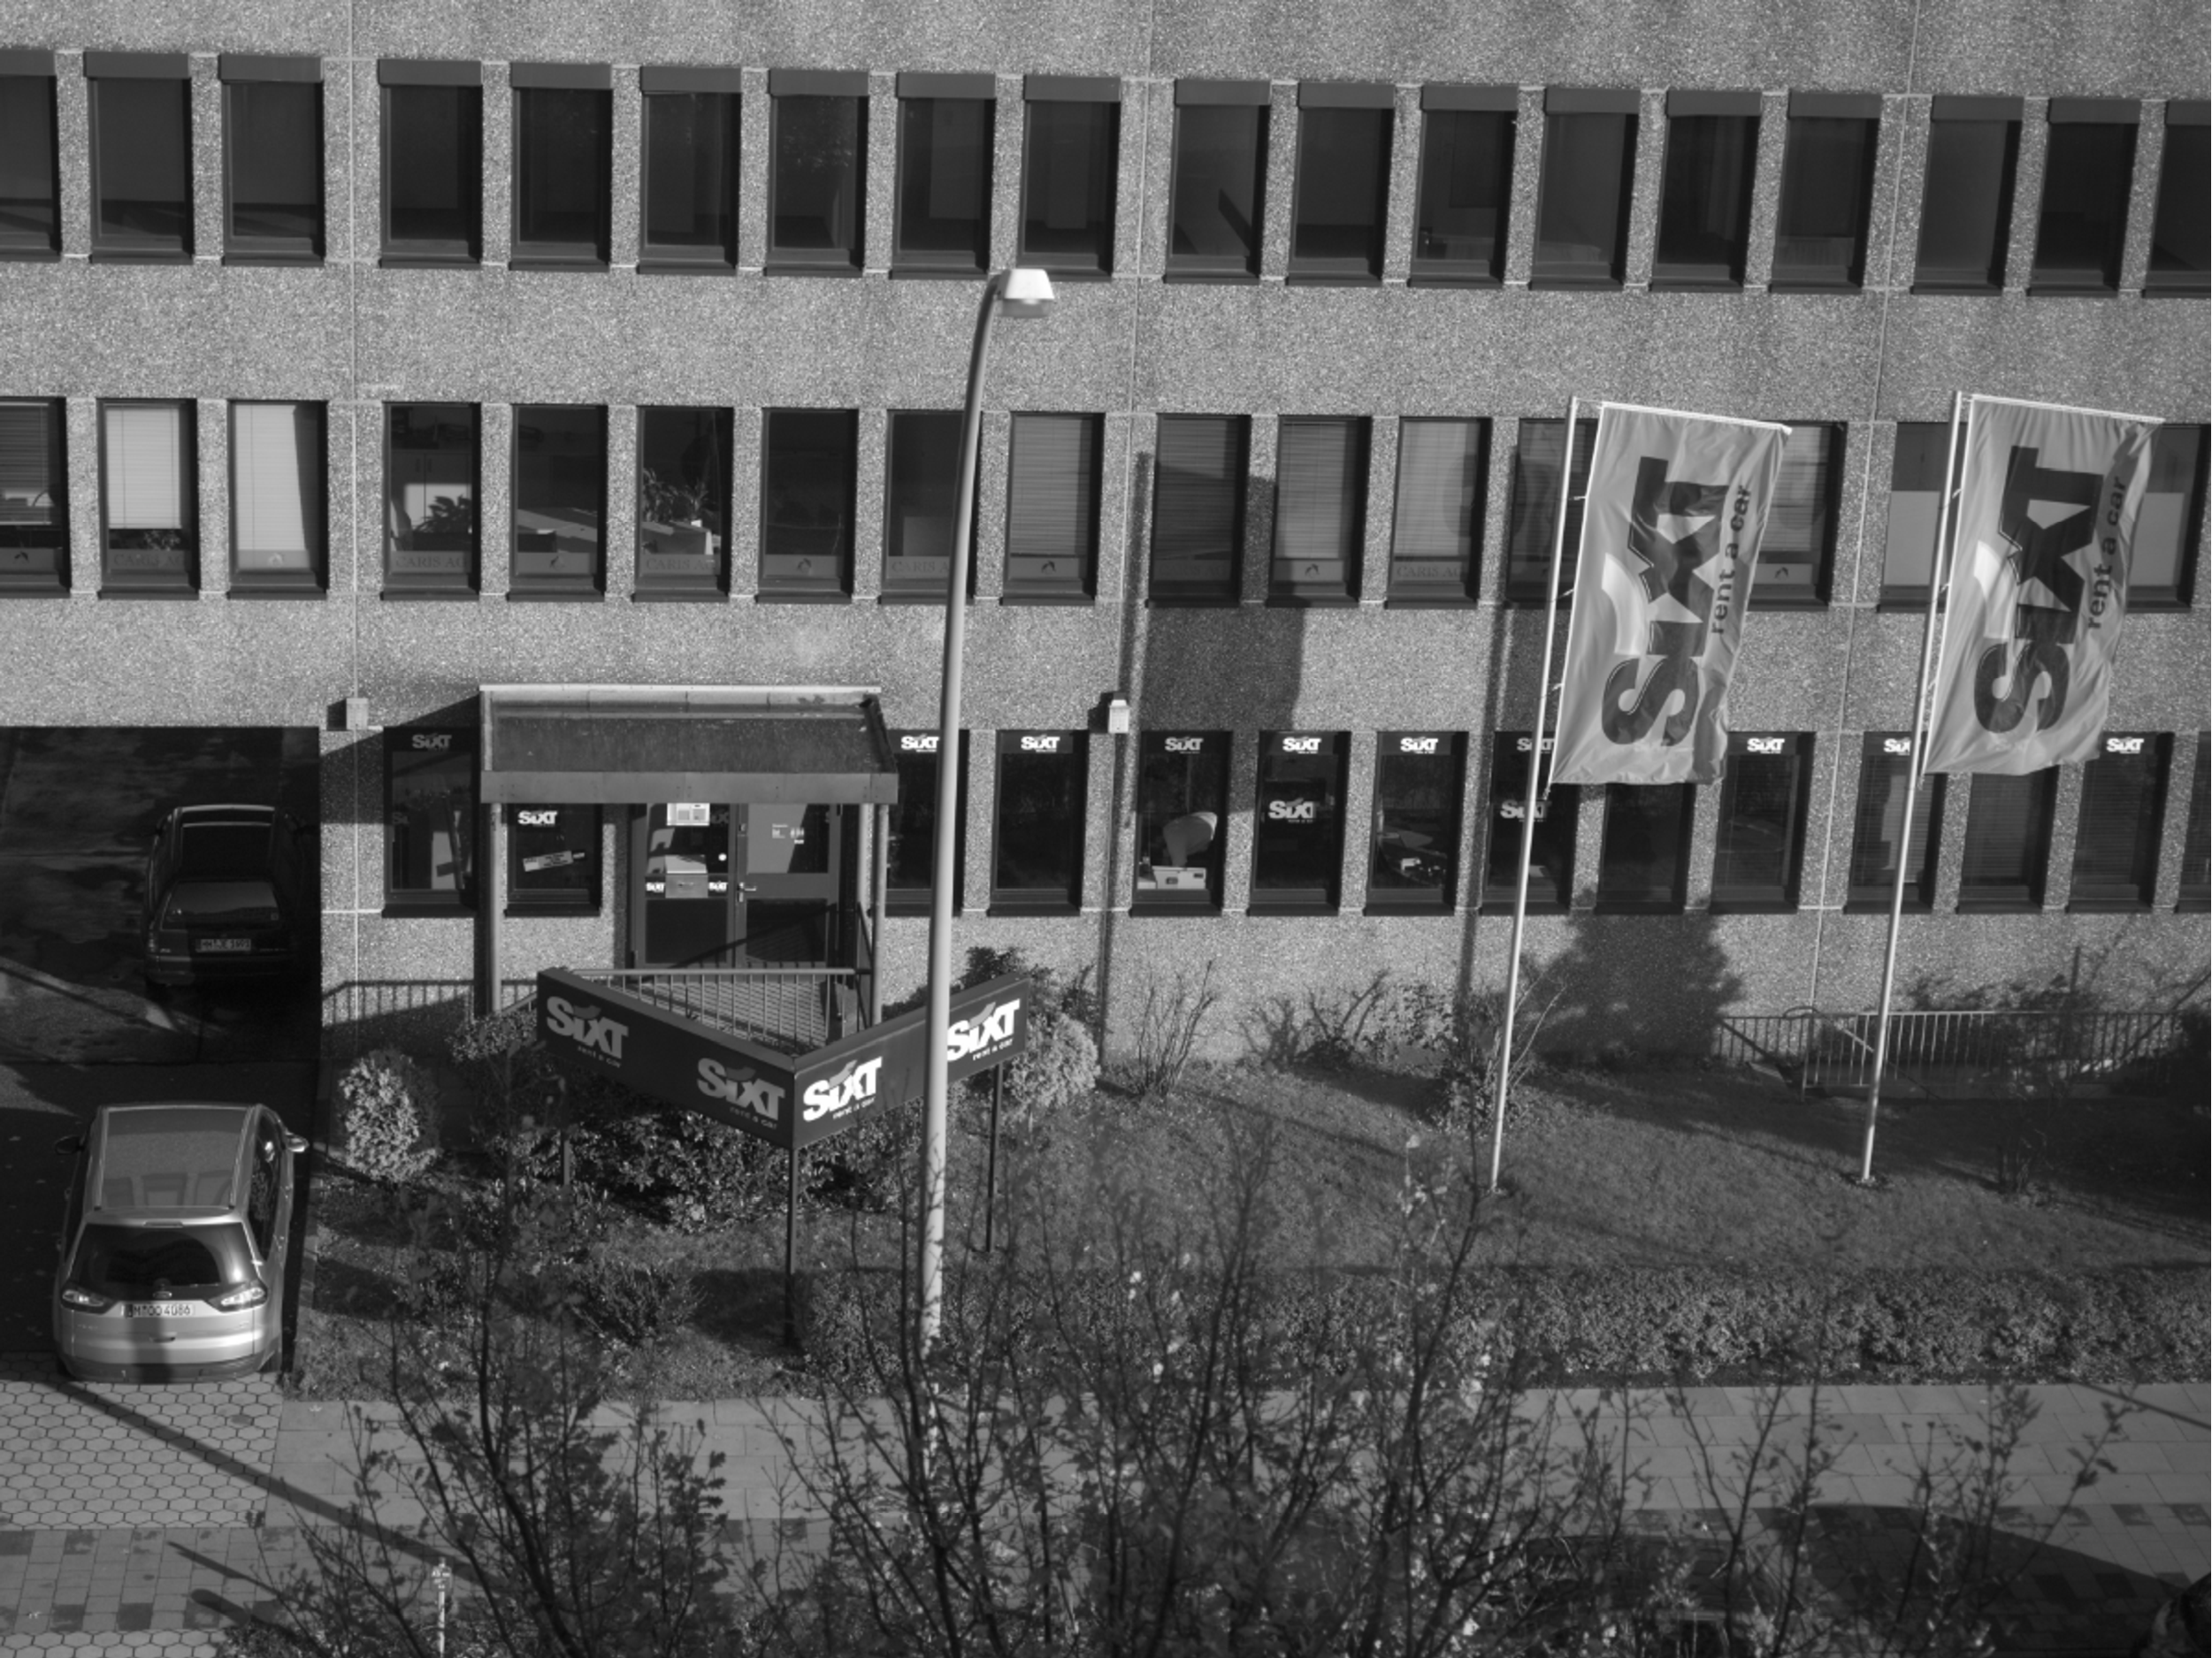
\includegraphics[scale=0.29]{images/big_building} 
\caption{\texttt{big\_building}, originale}
\end{figure}

\begin{figure}[!ht]
\centering
\includegraphics[scale=0.026]{{{images/big_building.bmpcut}}}
\caption{\texttt{big\_building}, taglio frequenze $< 5000$}
\end{figure}

\clearpage

Una cosa interessante da far notare è che il passaggio del taglio delle frequenze della trasformata è decisamente meno performante della procedura specificata dallo standard JPEG sul fronte della compressione della dimensione dell'immagine. Ad esempio, per \texttt{flower\_feveon.bmp}, un taglio delle frequenze al di sotto del valore 30 (che comporta un peggioramento della qualità dell'immagine ben visibile ad occhio nudo, anche in assenza di zoom) comprime l'immagine originale di un modesto 34\% (4.1 MB vs 2.7 MB).
\end{document}












